%%%%%%%%%%%%%%%%%%%%%% Procesadores CMP: usando la vectorización y la paralelización - EJERCICIO 2 %%%%%%%%%%%%%%%%%%%%%%
\newpage
\section{Ejercicio 2}
\subsection{Enunciado}
\begin{ejer}
    \textbf{2.-} En el directorio \texttt{paralelización} hay un pequeño programa que simula la propagación del 
    calor en una superficie rectangular. Se supone que la temperatura de cada uno de los bordes de la
    superficie se mantiene constante y el programa calcula la temperatura final de cada punto de
    la superficie representada como una matriz. Para ello utiliza un algoritmo iterativo tipo \texttt{stencil},
    el cual actualiza cada uno de los elementos de la matriz en función del valor previo del mismo
    elemento y sus vecinos.
    \par El código principal del algoritmo se encuentra en el fichero \texttt{heat.cpp}, que será el único que se
    necesitará modificar. Además, el fichero \texttt{matrix.h} proporciona un tipo de datos para almacenar las
    matrices utilizadas por el algoritmo, mientras que el fichero \texttt{main.cpp} incluye el código necesario
    para ejecutar el programa y medir el tiempo empleado en realizar la simulación. El programa permite
     configurar múltiples parámetros de la ejecución mediante opciones de la línea de comandos 
     (ver \texttt{main.cpp}).
    \par Además del programa, se incluye un \texttt{Makefile} para compilarlo usando tanto el compilador \texttt{GCC}
    como el \texttt{ICC}. Se incluyen también scripts para automatizar la comprobación de que los resultados
    son correctos y para automatizar la medida del tiempo de ejecución del programa usando diferente
    número de hilos (generando ficheros \texttt{tsv} que se pueden utilizar para generar gráficas fácilmente
    con multitud de programas, incluyendo cualquier hoja de cálculo). Se aconseja el uso de un
    ordenador que tenga 4 cores o más. Finalmente, se incluyen tres casos de prueba y su salida
    correspondiente, que se utilizarán para comprobar la corrección del programa modificado y para
    medir su rendimiento. El \texttt{Makefile} incluye objetivos para ejecutar todos los tests
    (\texttt{make tests} o \texttt{make tests-icc}) y para realizar la toma de tiempos (\texttt{make times} o
     \texttt{make times-icc}).
    \par Para completar este ejercicio, realiza lo siguiente:
    \begin{itemize}
        \item El procedimiento \texttt{solve} de \texttt{heat.cpp} tiene 3 bucles. Identifícalos y explica para cada uno
        de ellos si es candidato para la paralelización usando OpenMP. Indica en cada caso qué
        \texttt{pragma} (o \texttt{pragmas}) sería necesario añadir para realizar la paralelización correctamente.
        Presta especial cuidado a la clasificación de las variables (ya sean de reducción, compartidas
        o privadas).
        \item Prueba a paralelizar individualmente cada uno de los bucles paralelizables y prueba también a
        paralelizar todos los bucles paralelizables a la vez. Para cada versión resultante del programa,
        mide el tiempo de ejecución con diferente número de hilos de cada uno de los tres casos de
        prueba incluidos y genera las correspondientes gráficas mostrando el tiempo de ejecución y
        la escalabilidad obtenida (similar a las figuras \ref{fig:p2enun2-1} y \ref{fig:p2enun2-2}). Comenta los resultados.
    \end{itemize}
\end{ejer}
 %%% IMÁGENES %%%
\begin{figure}[H]
    \centering
    \subfigure[Tiempo de ejecución vs nº de hilos]{
        \label{fig:p2enun2-1}
        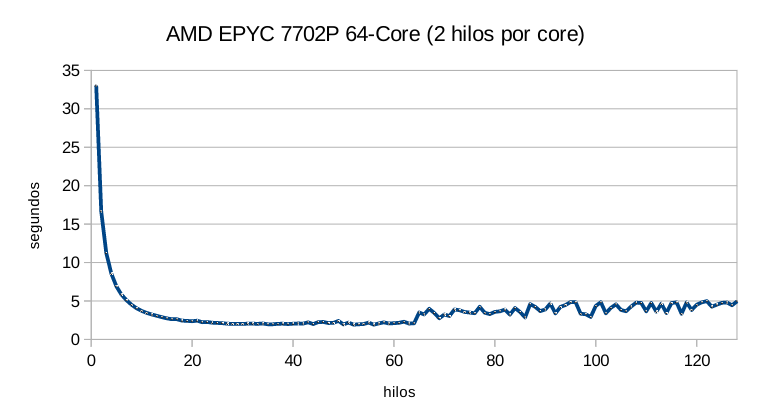
\includegraphics[width=0.45\textwidth]{p2enun2-1}}
    \subfigure[Escalabilidad de la aplicación]{
        \label{fig:p2enun2-2}
        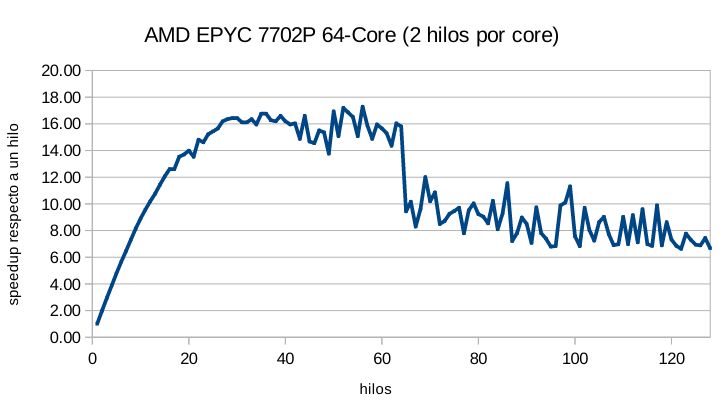
\includegraphics[width=0.45\textwidth]{p2enun2-2}}
\end{figure}
\subsection{Desarrollo}
